\subsection{Kommunikation}\label{subsec: Kommunikation} \todo{anpassen}
\subsubsection{WLAN Konfiguration}\label{subsub: Wlan Konfiguration}
Die Funkkommunikation zwischen Sensor, Aktor und MQTT-Brocker wird mittels Wireless Local Area Network (WLAN) auf dem OSI layer 1 stattfinden. Um die einzelnen Target also Sensoren und Aktoren in das Lokale Netzwerk zu verbinden, wird beim Starten des ESP32 ein Accespoint eröffnet. Für diesen WiFi-Manager Prozess wird eine Bibliothek eingebunden. Die benötigte Bibliothek steht auf Github zur Verfügung \cite{zhouhan0126_zhouhan0126/wifimanager-esp32_2019}. 

\begin{figure}[H]
	\centering
	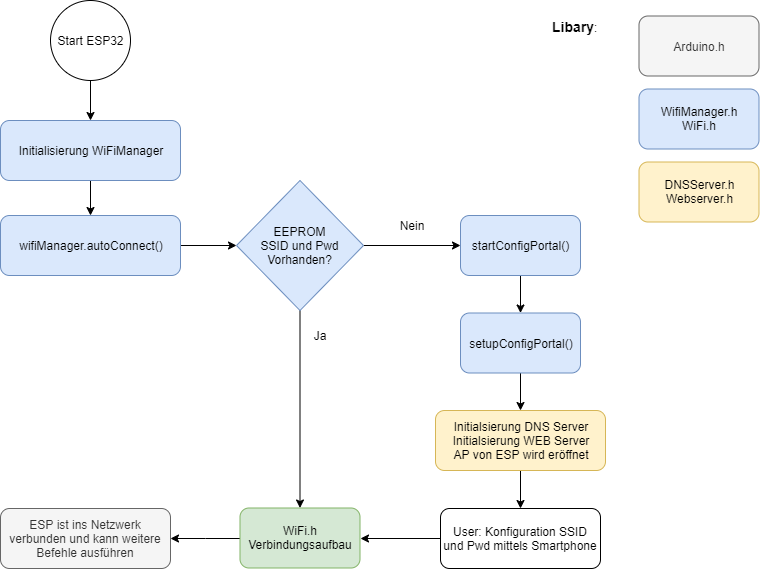
\includegraphics[width=\textwidth]{graphics/statediagramWiFi.png}
	\caption{Statediagram Verbindungsaufbau ESP ins Netzwerk mit einem AP}
	\label{pic: statediagramWiFi}
\end{figure}   

Wird die Bibliothek WiFiManager.h eingebunden und initialisiert stehen verschiedene Funktionen zur Verfügung. Die Funktion autoConnect() eröffnet nach dem Start des ESP einen Access Point wenn keine Konfigurationsdaten im nichtflüchtigen Speicher vorhanden sind. Falls Konfigurationsdaten vorhanden sind werden sie aus dem EEPROM gelesen und es wird kein Access Point eröffnet. Sollen aber die Konfigurationen bei jedem Start durchgeführt werden, kann die Funktion startConfigPortal() aufgerufen werden.   

Der Acces Point kann bei bedarf auch passwortgeschützt verwendet werden. In diesem Versuch wird er ohne Passwort genutzt und ist somit mit einem Smartphone oder Notebook ersichtlich, siehe Abbildung \ref{pic: wifiNetz}. Wird kein Name zugewiesen, generiert der ESP selber ein Name mit ESP und Chip-ID.
\begin{figure}[H]
	\centering
	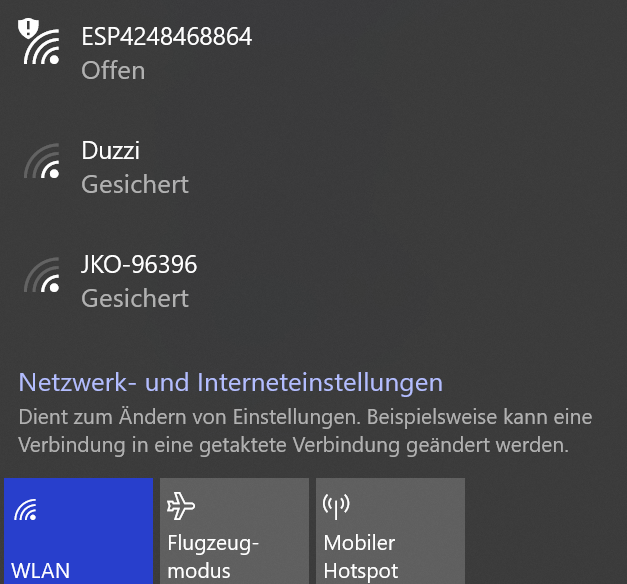
\includegraphics[width=0.5\textwidth]{graphics/WifiNetz.png}
	\caption{Esp Acces Point}
	\label{pic: wifiNetz}
\end{figure} 
Sobald "verbinden" mit diesem Netzwerk gewählt wird, startet der Browser eine Konfigurationsseite mit der IP Adresse des Targets. Nun ist ein Menü ersichtlich mit folgenden Wahlmöglichkeiten, siehe Abbildung \ref{pic: wifiNetz}:

\begin{figure}[H]
	\centering
	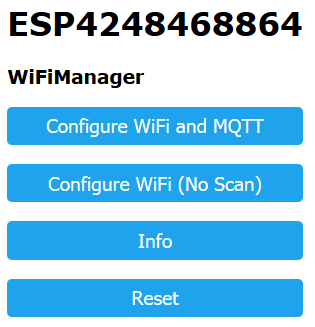
\includegraphics[width=0.5\textwidth]{graphics/WifiHome.png}
	\caption{Esp Konfiguration Home Menu}
	\label{pic: wifiHome}
\end{figure}   

Wird 'Configure WiFi and MQTT' angewählt erscheint folgende Ansicht in Abbildung \ref{pic: wifiKonfig}.

\begin{figure}[H]
	\centering
	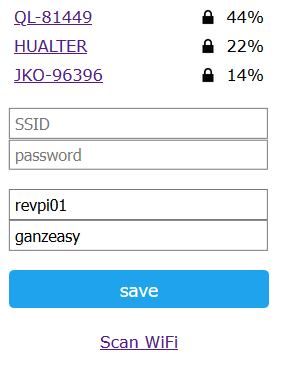
\includegraphics[width=0.5\textwidth]{graphics/WifiKonfig.png}
	\caption{Esp Konfiguration WiFi und MQTT}
	\label{pic: wifiKonfig}
\end{figure}   

Netzwerke, welche in der Umgebung gefunden wurden, werden angezeigt, die Parameter die zur WiFi Verbindung notwendig sind, können nun eingegeben werden. Im unteren Teil wird eine Voreinstellung der MQTT-Brocker-Adresse angezeigt und dessen Passwort, diese können beliebig geändert werden. Im WiFiManager Hauptmenü können die gleichen Konfigurationen ohne, dass nach vorhandenen Netzen gesucht wird, mit dem 'Configure WiFi(No Scan)' Button, gemacht werden. Mit dem Info Button werden Folgende Informationen angezeigt ChipID, Soft AP IP und Soft AP MAC wie auch Station AP MAC Adresse.

\begin{figure}[H]
	\centering
	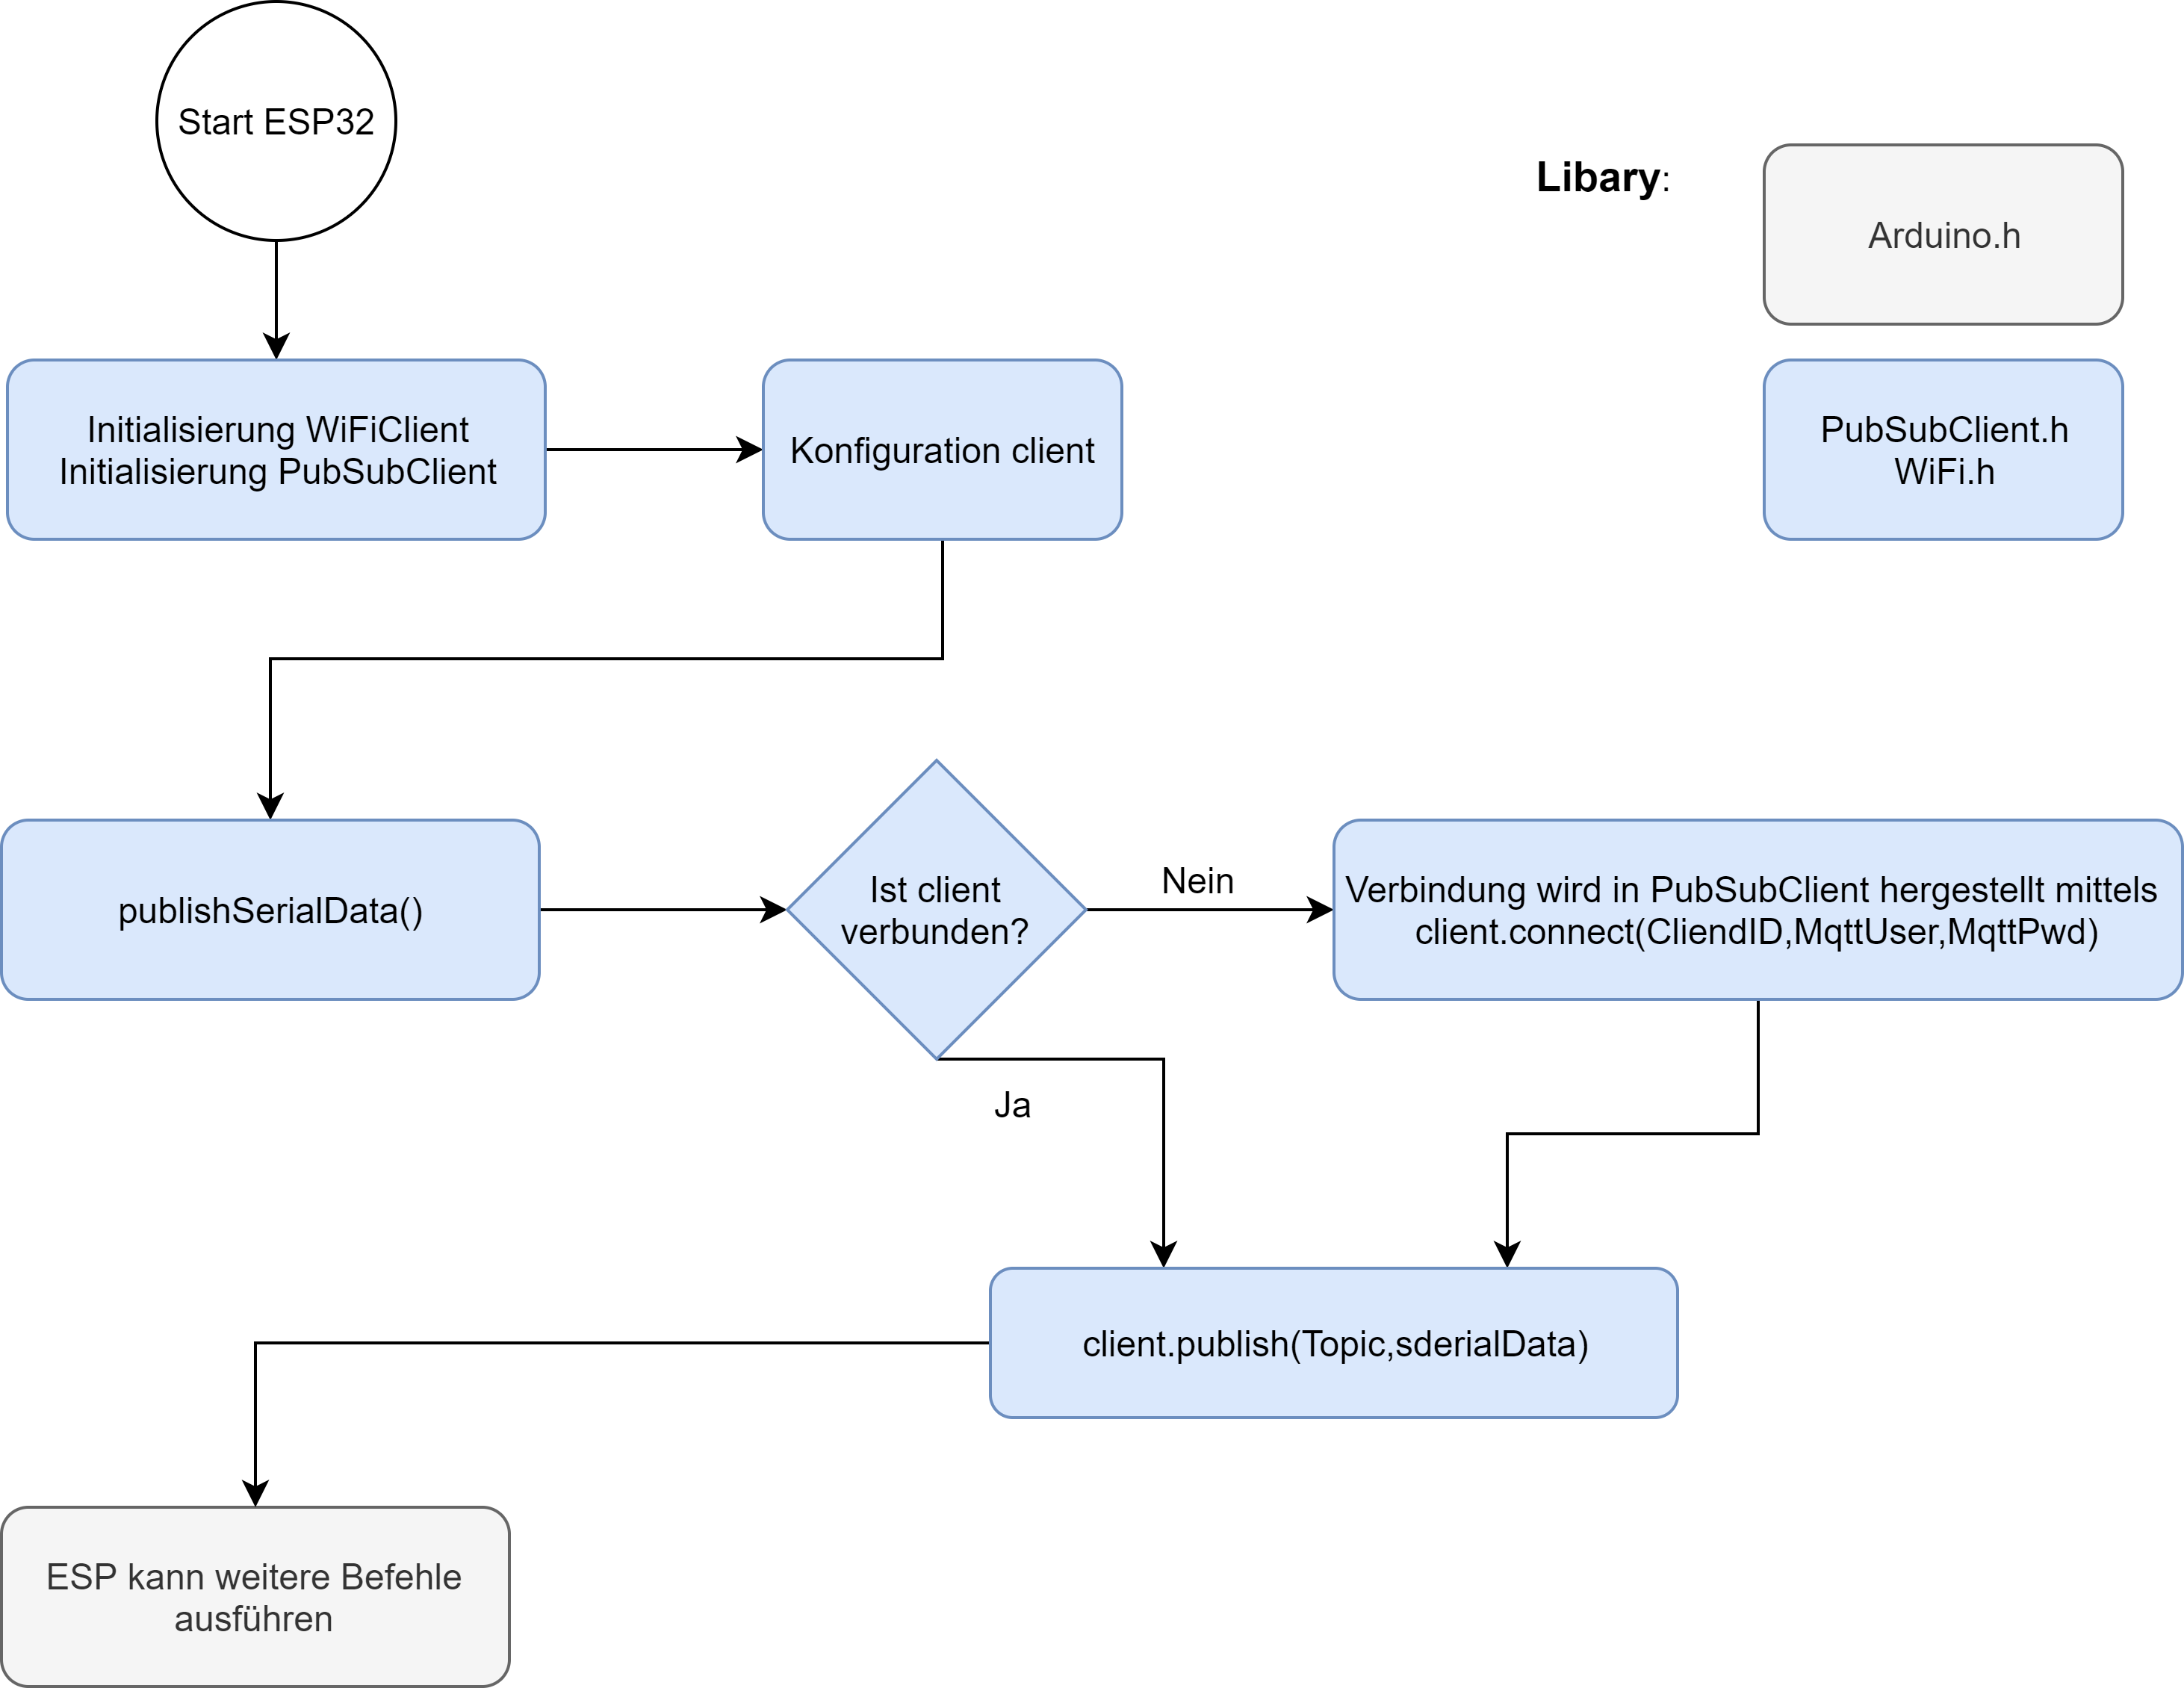
\includegraphics[width=\textwidth]{graphics/MQTTSubPubClient.png}
	\caption{Esp Info}
	\label{pic: SubPubClient}
\end{figure}   

Die für die MQTT-Kommunikation wird die Libary PubSubClient.h eingebunden. Als erstes wird der WiFiClient initialisiert. 

Danach wird der PubSubClinet als Client instantiiert, für diesen Vorgang werden folgende Parameter benötigt:\\
\begin{itemize}
\item 	server: Adresse von MQTT-Server\\
\item 	port: der Port von dem MQTT-Server\\
\item 	client: eine Instanz vom Ethernet-Client.\\
\end{itemize}
Die Funktion publishSerialData() ermöglicht, eine Nachricht zu veröffentlichen, bei diesem Vorgang wird den Topic und die seriellen Daten veröffentlicht. Beim Aufruf dieser Funktion, wird jedes mal überprüft ob die Verbindung zum MQTT-Borcker in Ordnung ist. 

Ist die Verbindung nicht in Ordnung, wird sie mit der Funktion connect(), hergestellt. Um diesen Prozess erfolgreich durch zu führen werden, CliendID, MQTT-Benutzername und Passwort benötigt.

Ist die Verbindung in Ordnung werden die Daten mit dem Befehl publish() veröffentlicht \cite{noauthor_arduino_nodate-1}.

\subsubsection{Lizenzen} \todo{anpassen auf github min 1 ganze Seite, veröffentlichen usw}
Die Bibliotheken welche in den Kapiteln \ref{subsub: Wlan Konfiguration} , \ref{subsec: Framework} erwähnt wurden, sind freie Softwarepakete und können unter der Bedingung der GNU Lesser General Public Lizenz (LGPL) geändert werden. Die LGPL gibt die Freiheit das Programm, für jeden Zweck auszuführen, anzupassen und die Änderungen zu veröffentlichen. \cite{noauthor_gnu.org_nodate}.
 
